\documentclass[12pt, twoside]{report}
\usepackage{blindtext}
\usepackage[utf8]{inputenc}
\usepackage{graphicx}
\graphicspath{{recursos/}}
\usepackage{float}
\usepackage[letterpaper,width=150mm,top=20mm,bottom=20mm,left=24mm,right=24mm,bindingoffset=0mm]{geometry}
\usepackage[section]{placeins}
\usepackage{booktabs}
\usepackage[spanish,es-nodecimaldot,es-tabla]{babel}
\usepackage{tikz} 
\usepackage{tocloft}
\usepackage{setspace}
%\usepackage{apacite}
%\usepackage{natbib}
%\bibliographystyle{abbrvnat}
%\setcitestyle{authoryear,open={(},close={)}}
\usepackage{filecontents}
\usepackage[nottoc]{tocbibind}
\usepackage{caption}
\usepackage{subcaption}
\usepackage{threeparttable}
\usepackage{acro}
\usepackage{dsfont}
\usepackage{lastpage}
\usepackage{makecell}
\usepackage{tasks}
\usepackage{fancyhdr}
\pagestyle{fancy}
\fancyhead{}
\fancyhead[RO,LE]{Control inteligente basado en navegación inercial para un brazo robótico articulado}
\fancyfoot{}
\fancyfoot[LE,RO]{\thepage}
\fancyfoot[CO,CE]{Nicolas Castañeda David Emmanuel}
\renewcommand{\headrulewidth}{0.4pt}
\renewcommand{\footrulewidth}{0.4pt} 
\usepackage{amsmath}
\usepackage{amssymb,amsthm,listings}
\usepackage{braket,lipsum,titlesec}
\usepackage{cleveref,setspace}
\makeatletter
\renewcommand*\env@matrix[1][*\c@MaxMatrixCols c]{%
  \hskip -\arraycolsep
  \let\@ifnextchar\new@ifnextchar
  \array{#1}}
\makeatother
\usepackage{dcolumn}
\newcolumntype{d}{D{-}{-}{0}}
\usepackage{xcolor}
\definecolor{Sepia}{RGB}{111,78,55}
\definecolor{Black}{RGB}{0,0,0}
\usepackage{setspace}
\usepackage{makeidx}
\makeindex
\usepackage{booktabs}
\usepackage{array}
\usepackage{cite}
\usepackage{gensymb}

\begin{document}

\newgeometry{top=10mm,bottom=5mm,left=0mm,right=0mm}

\thispagestyle{empty}
\begin{minipage}[c][0.17\textheight][c]{0.22\textwidth}
	\begin{center}
		
\includegraphics[scale=0.25]{logo-ipn-guinda.png}
	\end{center}
\end{minipage}
\begin{minipage}[c][0.195\textheight][c]{0.71\textwidth}
	\begin{center}
		\vspace{0.3cm}
		\textbf{\textsc{\Large INSTITUTO POLIT\'ECNICO NACIONAL}}
		\vspace{0.4cm}
		\color{Black}\hrule height1pt
		\vspace{0.2cm}
		{\color{Black}\hrule height1pt}
		\vspace{0.4cm}
		\color{Black}\textbf{\textsc{ESCUELA SUPERIOR DE INGENIER\'IA MEC\'ANICA Y EL\'ECTRICA}}
		\textbf{\textsc{Unidad Culhuac\'an\\}}
		\textsc{Ingenier\'ia en Computaci\'on}\\[0.5cm] %
	\end{center}
\end{minipage}

\begin{minipage}[c][0.81\textheight][t]{0.22\textwidth}
	\begin{center}
		\color{Black}\vrule width1pt height16cm 
		\vspace{5mm}
		\hskip2pt
		\color{Black}\vrule width1pt height16cm
		\hskip2mm
		\color{Black}\vrule width1pt height16cm \\
		\includegraphics[scale=0.14]{recursos/esime.png}
	\end{center}
\end{minipage}
\begin{minipage}[c][0.70\textheight][t]{0.7\textwidth}
	\begin{center}
		\vspace{1.5cm}
		
		{\Huge\scshape Control inteligente basado en navegaci\'on inercial para un brazo rob\'otico articulado}
		
		\vspace{3.5cm}            
		
		\textsc{\LARGE T E S I N A}\\[0.5cm]
		\textsc{\large que para obtener el t\'itulo de}\\[0.5cm]
		\textsc{\large Ingeniero en Computaci\'on}\\[0.5cm]
		\textsc{\large presenta}\\[0.5cm]
		\textsc{\large Nicolas Castañeda David Emmanuel}\\[2cm]          
		
		\vspace{1cm}
		
	\end{center}
	
	{\large\scshape Asesores:\\[0.3cm] {M. en C. Jos\'e Antonio Loaiza Brito\\ 
			Ing. Enrique Cisneros Sedano}}
	
	\vspace{0.5cm}
	
	\begin{flushright}
		\large{Ciudad de México, 16 de enero de 2024}
	\end{flushright}
\end{minipage}

\restoregeometry

\onehalfspacing

%\thispagestyle{empty}
\textbf{\Huge Agradecimientos}
\vspace{1cm}

Agradezco a mi asesor, José Antonio Loaiza Brito, por permitirme trabajar en un proyecto donde adquirí invaluables habilidades para aplicarlas en el desarrollo de mi carrera, y por guiar el trabajo para alcanzar el objetivo, que fue la titulación.\\
También agradezco a la empresa Sistemas Eléctricos de Potencia Computarizada (SEDPC), por los recursos económicos y materiales y la asesoría prestada para el desarrollo de este trabajo. En particular, quiero agradecer a los ingenieros Enrique Cisneros Sedano, Marco Emmanuel Toledano Polanco e Israel Flores Romero, quienes fueron responsables directos de mi proyecto y me sugirieron herramientas para llevarlo adelante.

\newpage
\thispagestyle{empty}
\textbf{\Huge Dedicatoria}
\vspace{1cm}

A mi incansable madre Fanny, que con su trabajo, su disciplina, sus consejos y su impulso me llevaron por el camino para completar mis estudios.\\
A mi hermana Mia Belén, la compañera con la que compartí los sinsabores y los triunfos de la vida por todos estos años.\\
A mi pareja, Ana, que me acompañó hasta el cansancio y me apoyó en todas las visitas a la empresa, durante el desarrollo de este trabajo.\\
A mis tíos Eder y Víctor, y mi abuela Violeta, que me apoyaron desde el momento en el que decidí estudiar en el Politécnico, y que a pesar de la pandemia, nunca se negaron a hacerlo.\\
Gracias por guiar mi vida, y ser el motivo de mi superación.

\newpage
\renewcommand{\contentsname}{\'Indice}
\tableofcontents

\newpage
\renewcommand{\listtablename}{Lista de tablas}
\listoftables

\newpage
\renewcommand{\listfigurename}{Lista de figuras}
\listoffigures

\newpage
\chapter{Anteproyecto}

\section{Introducci\'on}

Los brazos robóticos articulados son sistemas mecánicos con articulaciones rotativas, diseñados para replicar funciones del brazo humano, incluyendo movimientos de rotación y alcance. Suelen tener una pieza en el extremo del robot llamado efector final, como se muestra en la Figura \ref{fig:brazoR}, que realiza la función del robot en el entorno (soldar, manipular objetos, etc.). Cada unión en las articulaciones representa un grado de libertad (DoF).

\begin{figure}[htb]
	\centering
	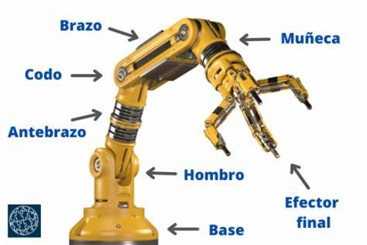
\includegraphics[scale=0.6]{brazo.jpg}
	\caption{Partes de un brazo robótico articulado de 3 DoF}
	\label{fig:brazoR}
\end{figure}

\newpage
Sistemas Eléctricos de Potencia Computarizada (SEPDC) es una empresa mexicana que se dedica a fabricar la serie Kaab de Controladores Lógicos Programables (PLC), computadoras especializadas para la automatización industrial (tienen inmunidad al ruido eléctrico y resistencia a la vibración y al impacto). Cada uno de ellos puede ser operado de forma remota a través de un software llamado SettDev. En la Figura \ref{fig:plc} se muestra el PLC-Kaab.

\begin{figure}[htb]
	\centering
	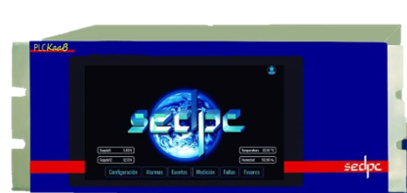
\includegraphics[scale=0.9]{plckaab.png}
	\caption{PLC-Kaab fabricado por SEDPC}
	\label{fig:plc}
\end{figure}

%\section{Planteamiento del problema}

Los brazos robóticos se han introducido rápidamente en la industria, sin embargo, aún existen desafíos para posicionar de manera precisa el brazo robótico que dificultan su introducción en industrias donde el manejo de las materias primas es delicado, sobre todo cuando dicho posicionamiento tiene que realizarse de manera autónoma.
\newline\newline\newline
Ubicar las articulaciones de un brazo para llegar a una posición deseada es un problema clásico de la robótica llamado cinemática inversa. Existen métodos algebraicos, geométricos e iterativos para resolverlo, sin embargo, dependen de la cantidad de grados de libertad del robot, además de que consumen una gran cantidad de recursos computacionales, lo que dificulta su uso en un sistema crítico.
\newpage
\section{Planteamiento del problema}

Los brazos robóticos se han introducido rápidamente en la industria, sin embargo, aún existen desafíos para posicionar de manera precisa el brazo robótico que dificultan su introducción en industrias donde el manejo de las materias primas es delicado, sobre todo cuando dicho posicionamiento tiene que realizarse de manera autónoma.
\newline\newline\newline
Ubicar las articulaciones de un brazo para llegar a una posición deseada es un problema clásico de la robótica llamado cinemática inversa. Existen métodos algebraicos, geométricos e iterativos para resolverlo, sin embargo, dependen de la cantidad de grados de libertad del robot, además de que consumen una gran cantidad de recursos computacionales, lo que dificulta su uso en un sistema crítico.

%\section{Objetivo general}

Desarrollar e implementar un sistema crítico de control, por medio de una Raspberry Pi, sensores inerciales y una red neuronal entrenada con aprendizaje no supervisado, para controlar la posición del efector final de un brazo robótico.

\newpage
\section{Objetivos específicos}
\begin{itemize}
	
	\item Desarrollar e implementar un programa en C++, utilizando los ángulos de inclinación en los tres ejes obtenidos por los sensores MPU6050, para determinar la posición del sensor en el extremo de la ortesis de brazo.
	
	\item Implementar la comunicación entre la Raspberry Pi y el software SettDev por medio de sockets TCP en C++ y C\# para enviar los ángulos de inclinación calculados al software, para poder guardar los datos y permitir reproducirlos en la simulación en 3D de un brazo robótico.
	
	\item Desarrollar e implementar una interfaz gráfica de usuario utilizando una pantalla táctil por medio del framework Qt para visualizar la cinemática inversa del brazo robótico a controlar.
	
	\item Desarrollar e implementar en SettDev la comunicación entre el módulo del brazo robótico en 3D y el PLC por medio de sockets UDP en C\# para enviar los ángulos de inclinación al controlador y reproducir los ángulos de inclinación en los servomotores posicionales.
	
	\item Implementar un sistema de inferencia neuro-difuso adaptativo (red neuronal ANFIS) utilizando C++ para resolver el problema de la cinemática inversa del brazo.
	
	\item Desarrollar e implementar un algoritmo de aprendizaje no supervisado utilizando C++ para entrenar la red neuronal.
	
\end{itemize}
\newpage
\section{Objetivo general}

Desarrollar e implementar un sistema crítico de control, por medio de una Raspberry Pi, sensores inerciales y una red neuronal entrenada con aprendizaje no supervisado, para controlar la posición del efector final de un brazo robótico.

\newpage
\section{Objetivos específicos}
\begin{itemize}
	
	\item Desarrollar e implementar un programa en C++, utilizando los ángulos de inclinación en los tres ejes obtenidos por los sensores MPU6050, para determinar la posición del sensor en el extremo de la ortesis de brazo.
	
	\item Implementar la comunicación entre la Raspberry Pi y el software SettDev por medio de sockets TCP en C++ y C\# para enviar los ángulos de inclinación calculados al software, para poder guardar los datos y permitir reproducirlos en la simulación en 3D de un brazo robótico.
	
	\item Desarrollar e implementar una interfaz gráfica de usuario utilizando una pantalla táctil por medio del framework Qt para visualizar la cinemática inversa del brazo robótico a controlar.
	
	\item Desarrollar e implementar en SettDev la comunicación entre el módulo del brazo robótico en 3D y el PLC por medio de sockets UDP en C\# para enviar los ángulos de inclinación al controlador y reproducir los ángulos de inclinación en los servomotores posicionales.
	
	\item Implementar un sistema de inferencia neuro-difuso adaptativo (red neuronal ANFIS) utilizando C++ para resolver el problema de la cinemática inversa del brazo.
	
	\item Desarrollar e implementar un algoritmo de aprendizaje no supervisado utilizando C++ para entrenar la red neuronal.
	
\end{itemize}

%\section{Justificación}

El sistema permitirá implementar un nuevo método para resolver la cinemática directa de forma trigonométrica a través de la navegación inercial, además de implementar un método que no dependa de la cantidad de grados de libertad del robot. Asimismo, será una aplicación práctica de las investigaciones previas a este trabajo sobre redes neuronales para el control de un brazo robótico.
\newpage
\section{Justificación}

El sistema permitirá implementar un nuevo método para resolver la cinemática directa de forma trigonométrica a través de la navegación inercial, además de implementar un método que no dependa de la cantidad de grados de libertad del robot. Asimismo, será una aplicación práctica de las investigaciones previas a este trabajo sobre redes neuronales para el control de un brazo robótico.

%\newpage
\section{Estado del arte}

\begin{table}[htb]
	\caption{Estado del arte}
	\centering
	\begin{tabular}{p{3.8cm}p{3.8cm}p{3.8cm}p{3.8cm}}
		\textbf{Título} & \textbf{Autores} & \textbf{Tipo de publicación, lugar y fecha} & \textbf{Descripción} \\ 
		\midrule
		FIKA: A Conformal Geometric Algebra Approach to a Fast Inverse Kinematics Algorithm for an Anthropomorphic Robotic Arm \newline\newline
		FIKA: Un enfoque de álgebra geométrica conforme para un eficaz algoritmo cinemático inverso para un brazo robótico antropomórfico &  
		Oscar Carbajal-Espinosa; Leobardo Campos-Macías; Miriam Díaz-Rodríguez \newline\newline
		Instituto Tecnológico y de Estudios Superiores de Monterrey; Intel Corporation; Tecnológico Nacional de México & 
		\begin{center}Artículo \par 
\includegraphics[width=3cm]{mexico.jpg} \par Mexico \par 2024\end{center} & 
		Propone un método geométrico iterativo de 3 fases para resolver el problema de la cinemática inversa.\newline\newline
		Sin embargo, requiere un tiempo de procesamiento de datos inaceptable en un sistema crítico.\\
		\midrule
		Implementation of singularity-free inverse kinematics for humanoid robotic arm using Bayesian optimized deep neural network. \newline\newline
		Implementación de cinemática inversa sin singularidad para brazo robótico humanoide utilizando una red neuronal profunda optimizada por métodos Bayesianos. &  
		Omur Aydogmus; Gullu Boztas \newline\newline 
		Firat University & 
		\begin{center}Artículo \par 
\includegraphics[width=3cm]{turquia.png} \par Turquía \par 2024\end{center} & 
		Utiliza una red neuronal basada en aprendizaje profundo para resolver la cinemática inversa en una simulación.\newline\newline Sin embargo, el proyecto no se llevó a una aplicación práctica. \\
	\end{tabular}
\end{table}

\newpage
\begin{table}[htb]
	\caption{Estado del arte (continuación)}
	\centering
	\begin{tabular}{p{3.8cm}p{3.8cm}p{3.8cm}p{3.8cm}}
		\textbf{Título} & \textbf{Autores} & \textbf{Tipo de publicación, lugar y fecha} & \textbf{Descripción} \\ 
		\midrule
		Inverse kinematics solution and control method of 6-degree-of-freedom manipulator based on deep reinforcement learning. \newline\newline
		Solución de cinemática inversa y método de control de un manipulador de 6 grados de libertad basado en aprendizaje de refuerzo profundo. &  
		Chengyi Zhao; Yimin Wei; Junfeng Xiao; Yong Sun; Dongxing Zhang; Qiuquan Guo; Jun Yang \newline\newline 
		University of Electronic Science and Technology of China & 
		\begin{center}Artículo \par 
\includegraphics[width=3cm]{china.png} \par China \par 2024\end{center} & 
		Propone un algoritmo de aprendizaje por refuerzo que calcula la distancia entre el efector final y la posición deseada. \newline\newline Sin embargo, se volverá ineficaz cuando se adapte a brazos de diferente longitud. \\
	\end{tabular}
\end{table}
\newpage
\newpage
\section{Estado del arte}

\begin{table}[htb]
	\caption{Estado del arte}
	\centering
	\begin{tabular}{p{3.8cm}p{3.8cm}p{3.8cm}p{3.8cm}}
		\textbf{Título} & \textbf{Autores} & \textbf{Tipo de publicación, lugar y fecha} & \textbf{Descripción} \\ 
		\midrule
		FIKA: A Conformal Geometric Algebra Approach to a Fast Inverse Kinematics Algorithm for an Anthropomorphic Robotic Arm \newline\newline
		FIKA: Un enfoque de álgebra geométrica conforme para un eficaz algoritmo cinemático inverso para un brazo robótico antropomórfico &  
		Oscar Carbajal-Espinosa; Leobardo Campos-Macías; Miriam Díaz-Rodríguez \newline\newline
		Instituto Tecnológico y de Estudios Superiores de Monterrey; Intel Corporation; Tecnológico Nacional de México & 
		\begin{center}Artículo \par 
\includegraphics[width=3cm]{mexico.jpg} \par Mexico \par 2024\end{center} & 
		Propone un método geométrico iterativo de 3 fases para resolver el problema de la cinemática inversa.\newline\newline
		Sin embargo, requiere un tiempo de procesamiento de datos inaceptable en un sistema crítico.\\
		\midrule
		Implementation of singularity-free inverse kinematics for humanoid robotic arm using Bayesian optimized deep neural network. \newline\newline
		Implementación de cinemática inversa sin singularidad para brazo robótico humanoide utilizando una red neuronal profunda optimizada por métodos Bayesianos. &  
		Omur Aydogmus; Gullu Boztas \newline\newline 
		Firat University & 
		\begin{center}Artículo \par 
\includegraphics[width=3cm]{turquia.png} \par Turquía \par 2024\end{center} & 
		Utiliza una red neuronal basada en aprendizaje profundo para resolver la cinemática inversa en una simulación.\newline\newline Sin embargo, el proyecto no se llevó a una aplicación práctica. \\
	\end{tabular}
\end{table}

\newpage
\begin{table}[htb]
	\caption{Estado del arte (continuación)}
	\centering
	\begin{tabular}{p{3.8cm}p{3.8cm}p{3.8cm}p{3.8cm}}
		\textbf{Título} & \textbf{Autores} & \textbf{Tipo de publicación, lugar y fecha} & \textbf{Descripción} \\ 
		\midrule
		Inverse kinematics solution and control method of 6-degree-of-freedom manipulator based on deep reinforcement learning. \newline\newline
		Solución de cinemática inversa y método de control de un manipulador de 6 grados de libertad basado en aprendizaje de refuerzo profundo. &  
		Chengyi Zhao; Yimin Wei; Junfeng Xiao; Yong Sun; Dongxing Zhang; Qiuquan Guo; Jun Yang \newline\newline 
		University of Electronic Science and Technology of China & 
		\begin{center}Artículo \par 
\includegraphics[width=3cm]{china.png} \par China \par 2024\end{center} & 
		Propone un algoritmo de aprendizaje por refuerzo que calcula la distancia entre el efector final y la posición deseada. \newline\newline Sin embargo, se volverá ineficaz cuando se adapte a brazos de diferente longitud. \\
	\end{tabular}
\end{table}

%\section{Marco teórico}

\subsection*{Raspberry Pi 3 B+}
\begin{itemize}
	\item Funciona con un sistema operativo basado en la arquitectura ARM.
	\item Módulo Wi-Fi de banda dual de 2,4 y 5 GHz.
	\item 40 pines Entrada/Salida de Propósito General (GPIO)
	\item Salidas de 3.3 y 5 V, buses I²C, SPI
\end{itemize}

\begin{figure}[htb]
	\centering
	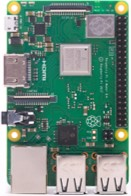
\includegraphics[scale=0.5]{raspberrypi.jpg}
	\caption{Raspberry Pi 3 B+}
\end{figure}

\subsection*{Qt}
\begin{itemize}
	\item Optimizada para aplicaciones con interfaces gráficas en sistemas embebidos.
	\item Soporte para C++
	\item Utiliza el lenguaje declarativo QML para programar la interfaz
\end{itemize}

\begin{figure}[htb]
	\centering
	
\includegraphics[scale=0.5]{qt.jpg}
	\caption{Logotipo de Qt Framework}
\end{figure}

\subsection*{Bus I2C}
\begin{itemize}
	\item Bus serial de comunicación de tipo maestro-esclavo.
	\item Línea serial de datos bidireccional (SDA)  y línea serial de reloj (SCL).
	\item Espacio de direcciones, cada dirección identifica a un dispositivo conectado al bus.
\end{itemize}

\begin{figure}[htb]
	\centering
	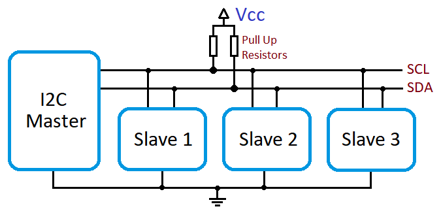
\includegraphics[scale=0.5]{i2c.png}
	\caption{Diagrama del bus I2C}
\end{figure}

\subsection*{Bus SPI}
\begin{itemize}
	\item Bus serial de comunicación de tipo maestro-esclavo.
	\item Líneas de entrada al esclavo (MOSI) y salida al esclavo (MISO), línea de reloj (SCLK).
	\item Línea de selección del chip (SS).
\end{itemize}

\begin{figure}[htb]
	\centering
	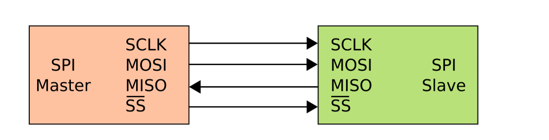
\includegraphics[scale=0.5]{spi.png}
	\caption{Diagrama del bus SPI}
\end{figure}

\subsection*{MPU-6050}
\begin{itemize}
	\item Giroscopio de vibración de Coriolis y acelerómetro de 3 ejes.
	\item Procesador de movimiento digital (DMP) que mide la orientación del sensor en tres ejes.
	\item Buffer FIFO interno.
	\item Filtro paso bajo.
	\item Comunicación por medio del bus I²C de hasta 400 KHz.
	\item Pin AD0 para cambiar la dirección en el bus. Solo puede tomar las direcciones 104 y 105.
\end{itemize}

\begin{figure}[htb]
	\centering
	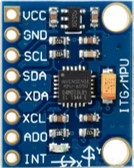
\includegraphics[scale=0.5]{mpu6050.jpg}
	\caption{Sensor inercial MPU6050}
\end{figure}

\subsection*{MPU-9250}
\begin{itemize}
	\item Giroscopio de vibración de Coriolis y acelerómetro de 3 ejes.
	\item Procesador de movimiento digital (DMP) que mide la orientación del sensor en tres ejes.
	\item Buffer FIFO interno.
	\item Filtro paso bajo.
	\item Comunicación por medio del bus SPI de hasta 10 MHz.
\end{itemize}

\begin{figure}[htb]
	\centering
	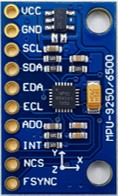
\includegraphics[scale=0.4]{mpu9250.jpg}
	\caption{Sensor inercial MPU9250}
\end{figure}

%\subsection*{Sensor flexible capacitivo}
%\begin{itemize}
%	\item Mide el ángulo de torsión al que se somete el sensor en una dirección.
%	\item El valor medido es una resistencia variable
%\end{itemize}

%\begin{figure}[htb]
%	\centering
%	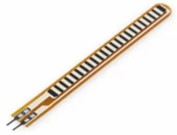
\includegraphics[scale=0.6]{flexsensor.jpg}
%	\caption{Sensor flexible capacitivo}
%\end{figure}

%\subsection*{Convertidor analógico-digital MCP3004}
%\begin{itemize}
%	\item Voltaje de referencia de 2,7 V a 5,5 V
%\end{itemize}

%\begin{figure}[htb]
%	\centering
%	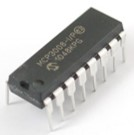
\includegraphics[scale=0.6]{mcp3004.jpg}
%	\caption{Convertidor A/D MCP3004}
%\end{figure}

\subsection*{Microservomotor posicional}
\begin{itemize}
	\item Ángulo de entrada de 0° a 180°
	\item Utiliza señales de modulación de ancho de pulso (PWM)
	\item Movimiento bidireccional
\end{itemize}

\begin{figure}[htb]
	\centering
	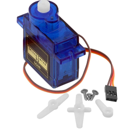
\includegraphics[scale=0.6]{servomotor.png}
	\caption{Microservomotor posicional}
\end{figure}
\newpage
\section{Marco teórico}

\subsection*{Raspberry Pi 3 B+}
\begin{itemize}
	\item Funciona con un sistema operativo basado en la arquitectura ARM.
	\item Módulo Wi-Fi de banda dual de 2,4 y 5 GHz.
	\item 40 pines Entrada/Salida de Propósito General (GPIO)
	\item Salidas de 3.3 y 5 V, buses I²C, SPI
\end{itemize}

\begin{figure}[htb]
	\centering
	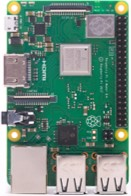
\includegraphics[scale=0.5]{raspberrypi.jpg}
	\caption{Raspberry Pi 3 B+}
\end{figure}

\subsection*{Qt}
\begin{itemize}
	\item Optimizada para aplicaciones con interfaces gráficas en sistemas embebidos.
	\item Soporte para C++
	\item Utiliza el lenguaje declarativo QML para programar la interfaz
\end{itemize}

\begin{figure}[htb]
	\centering
	
\includegraphics[scale=0.5]{qt.jpg}
	\caption{Logotipo de Qt Framework}
\end{figure}

\subsection*{Bus I2C}
\begin{itemize}
	\item Bus serial de comunicación de tipo maestro-esclavo.
	\item Línea serial de datos bidireccional (SDA)  y línea serial de reloj (SCL).
	\item Espacio de direcciones, cada dirección identifica a un dispositivo conectado al bus.
\end{itemize}

\begin{figure}[htb]
	\centering
	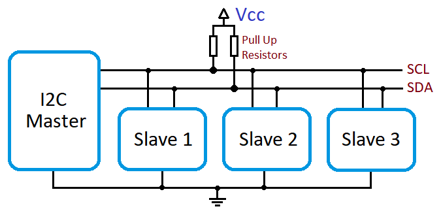
\includegraphics[scale=0.5]{i2c.png}
	\caption{Diagrama del bus I2C}
\end{figure}

\subsection*{Bus SPI}
\begin{itemize}
	\item Bus serial de comunicación de tipo maestro-esclavo.
	\item Líneas de entrada al esclavo (MOSI) y salida al esclavo (MISO), línea de reloj (SCLK).
	\item Línea de selección del chip (SS).
\end{itemize}

\begin{figure}[htb]
	\centering
	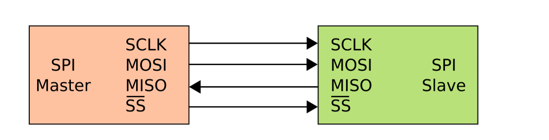
\includegraphics[scale=0.5]{spi.png}
	\caption{Diagrama del bus SPI}
\end{figure}

\subsection*{MPU-6050}
\begin{itemize}
	\item Giroscopio de vibración de Coriolis y acelerómetro de 3 ejes.
	\item Procesador de movimiento digital (DMP) que mide la orientación del sensor en tres ejes.
	\item Buffer FIFO interno.
	\item Filtro paso bajo.
	\item Comunicación por medio del bus I²C de hasta 400 KHz.
	\item Pin AD0 para cambiar la dirección en el bus. Solo puede tomar las direcciones 104 y 105.
\end{itemize}

\begin{figure}[htb]
	\centering
	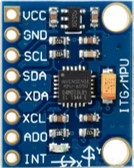
\includegraphics[scale=0.5]{mpu6050.jpg}
	\caption{Sensor inercial MPU6050}
\end{figure}

\subsection*{MPU-9250}
\begin{itemize}
	\item Giroscopio de vibración de Coriolis y acelerómetro de 3 ejes.
	\item Procesador de movimiento digital (DMP) que mide la orientación del sensor en tres ejes.
	\item Buffer FIFO interno.
	\item Filtro paso bajo.
	\item Comunicación por medio del bus SPI de hasta 10 MHz.
\end{itemize}

\begin{figure}[htb]
	\centering
	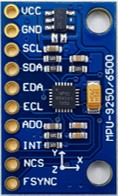
\includegraphics[scale=0.4]{mpu9250.jpg}
	\caption{Sensor inercial MPU9250}
\end{figure}

%\subsection*{Sensor flexible capacitivo}
%\begin{itemize}
%	\item Mide el ángulo de torsión al que se somete el sensor en una dirección.
%	\item El valor medido es una resistencia variable
%\end{itemize}

%\begin{figure}[htb]
%	\centering
%	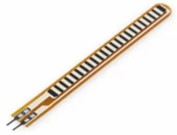
\includegraphics[scale=0.6]{flexsensor.jpg}
%	\caption{Sensor flexible capacitivo}
%\end{figure}

%\subsection*{Convertidor analógico-digital MCP3004}
%\begin{itemize}
%	\item Voltaje de referencia de 2,7 V a 5,5 V
%\end{itemize}

%\begin{figure}[htb]
%	\centering
%	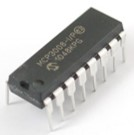
\includegraphics[scale=0.6]{mcp3004.jpg}
%	\caption{Convertidor A/D MCP3004}
%\end{figure}

\subsection*{Microservomotor posicional}
\begin{itemize}
	\item Ángulo de entrada de 0° a 180°
	\item Utiliza señales de modulación de ancho de pulso (PWM)
	\item Movimiento bidireccional
\end{itemize}

\begin{figure}[htb]
	\centering
	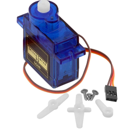
\includegraphics[scale=0.6]{servomotor.png}
	\caption{Microservomotor posicional}
\end{figure}

%\newpage
\section{Propuesta de solución}

\begin{figure}[htb]
	\centering
	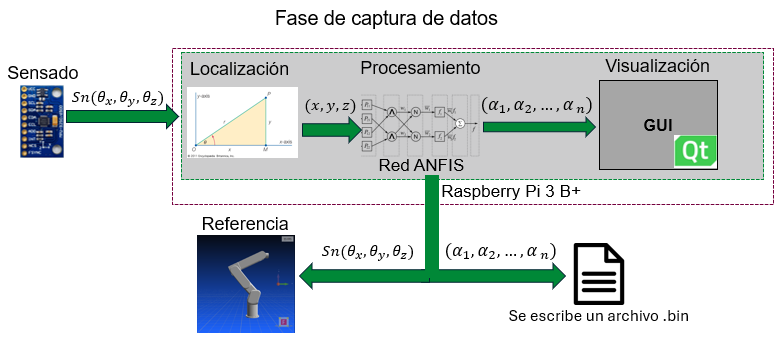
\includegraphics[scale=0.85]{fasecaptura.png}
	\caption{Etapa de captura de datos}
\end{figure}

\begin{figure}[htb]
	\centering
	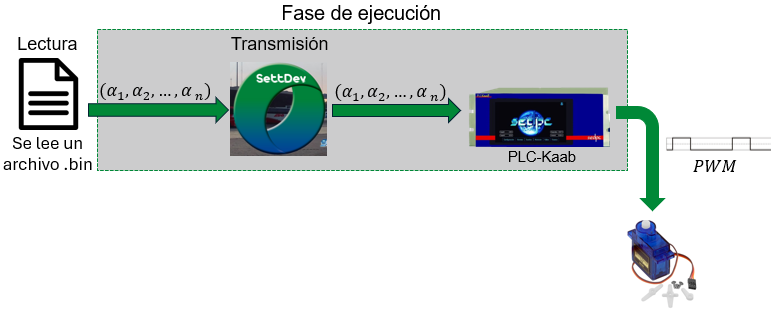
\includegraphics[scale=0.85]{faseejecucion.png}
	\caption{Fase de ejecución}
\end{figure}
\newpage
\newpage
\section{Propuesta de solución}

\begin{figure}[htb]
	\centering
	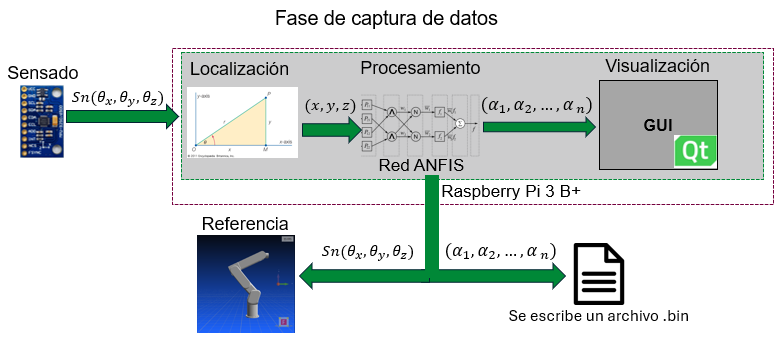
\includegraphics[scale=0.85]{fasecaptura.png}
	\caption{Etapa de captura de datos}
\end{figure}

\begin{figure}[htb]
	\centering
	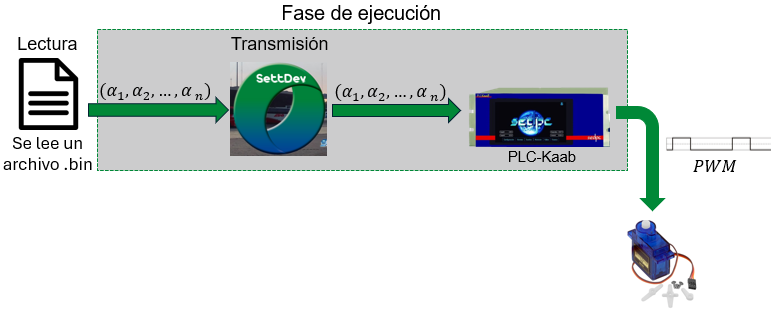
\includegraphics[scale=0.85]{faseejecucion.png}
	\caption{Fase de ejecución}
\end{figure}

\newpage
\chapter{Desarrollo del proyecto}

\section{Fase de captura de datos}

\subsection{Sensado}

La empresa requirió que se utilizara una ortesis de brazo donde se montara el sistema de medición de los sensores inerciales y la Raspberry Pi. La Figura \ref{fig:ortesis} muestra la ortesis de brazo utilizada. Para encontrar la posición del efector final, se utilizaron los dos sensores MPU-6050; uno se colocó en el codo, mientras que el segundo se colocó en el extremo de la ortesis. El sensor MPU-9250 se colocó en la parte superior de la mano, para controlar el movimiento del efector final.

\begin{figure}[htb]
	\centering
	\rotatebox{90}{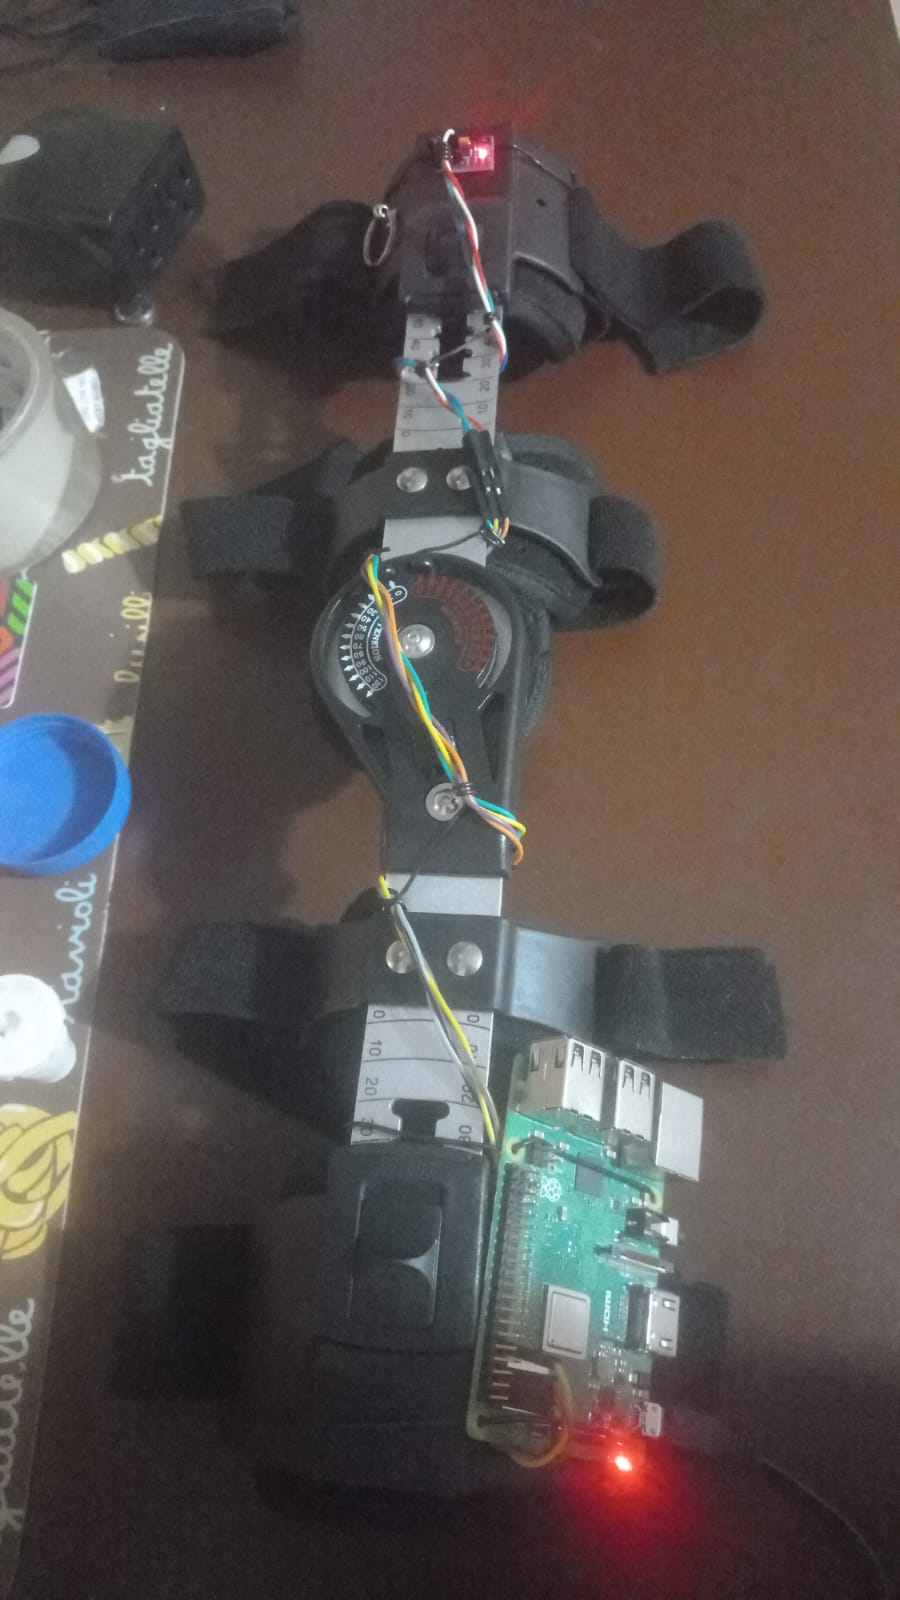
\includegraphics[scale=0.2]{ortesis.jpg}}
	\caption{Ortesis utilizada para el proyecto}
	\label{fig:ortesis}
\end{figure}

Se realizó la conexión entre los sensores y la Raspberry Pi 3 B+. La Figura \ref{fig:diagrama} muestra el diagrama de interconexión. Los pines SDA y SCL de los sensores MPU-6050 se conectaron al bus serial $I^2C$, mientras que los pines MISO, MOSI y SCK del sensor MPU-9250 se conectaron al bus serial SPI.

\begin{figure}[htb]
	\centering
	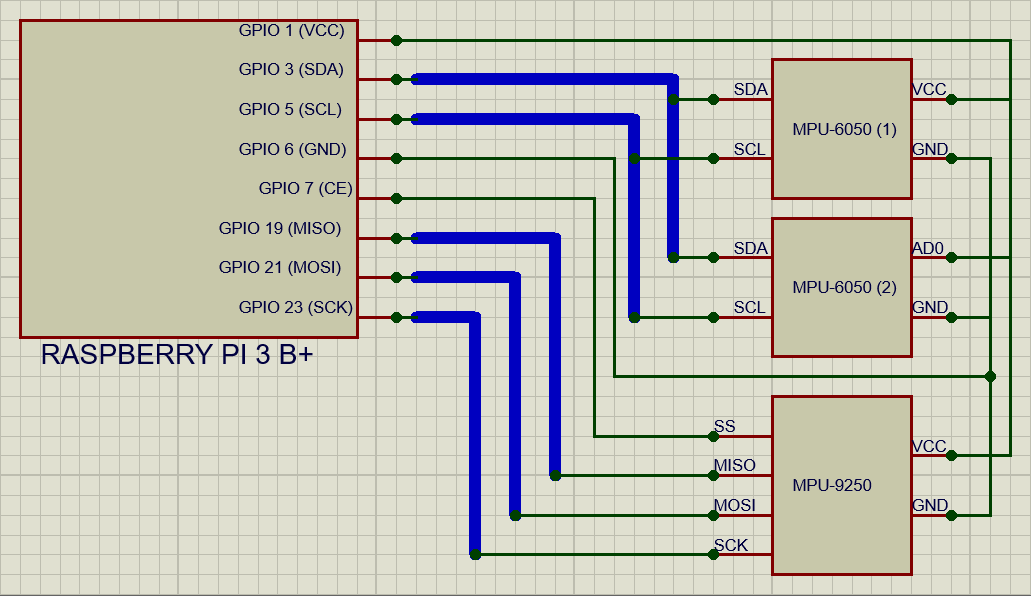
\includegraphics[scale=0.6]{diagrama.png}
	\caption{Diagrama de interconexión entre la Raspberry Pi y los sensores}
	\label{fig:diagrama}
\end{figure}

La línea SS del sensor MPU-9250 se conectó a la línea Chip Enable (CE) 1 de la Raspberry Pi. Nótese que tanto las líneas de datos (SDA), como las líneas de reloj (SCL) de los sensores MPU-6050, se conectaron a una única línea SDA o SCL, respectivamente, hacia la Raspberry Pi. Para evitar problemas de sincronización, se eligió la misma frecuencia de reloj para ambos sensores. Nótese también que se alimentó al sensor a través de la entrada AD0, en vez de VCC. Esto permite que su dirección en el bus $I^2C$ cambie de 104 a 105. Todos los sensores se alimentaron a través de la salida de voltaje de 3,3 V de la Raspberry Pi.

En lo que resta del documento, cuando se haga referencia a los sensores MPU-6050 y MPU-9250 en conjunto, se utilizará el prefijo MPU; cuando se haga referencia solo a uno de ellos, se hará con su nombre completo.

\subsubsection{Calibración}

Los sensores inerciales fabricados con tecnología MEMS, como los MPU, necesitan ser calibrados y tener un valor de referencia (offset) con el cual se corrija la orientación medida por el sensor \cite{offsetMPU}. El diagrama de la Figura \ref{fig:salidaMPU} obtenido del manual \cite{offsetMPU} muestra el proceso para obtener datos de los sensores MPU; los valores de referencia del acelerómetro y el giroscopio (Gyro and Accel Offset Registers) se aplican a las mediciones obtenidas por el giroscopio y el acelerómetro (Gyro and Accel MEMS), para corregir la mediciones y colocarlas en los registros del sensor (Gyro/Accel Output Registers). Luego, son procesadas por el Procesador de Movimiento Digital (DMP) y el resultado se almacena en un buffer FIFO interno.

\begin{figure}[htb]
	\centering
	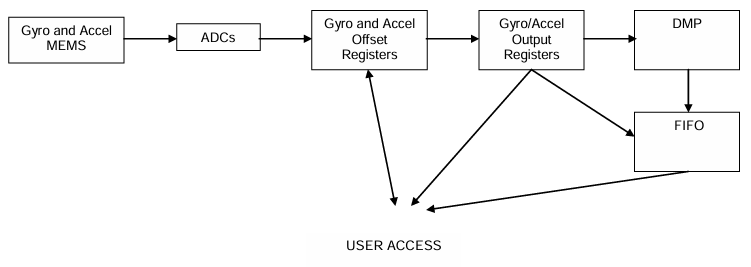
\includegraphics[scale=0.8]{salidaMPU.png}
	\caption{Lectura de datos de los sensores MPU}
	\label{fig:salidaMPU}
\end{figure}

%El buffer FIFO de los MPU permite implementar un patrón de arquitectura de segmentación de procesos (process pipeline); los datos obtenidos del DMP se colocan en un buffer interno del sensor de tipo FIFO (El primer dato que entra, es el último que sale), del cual se lee la orientación del sensor; esto permite que los datos de la orientación puedan ser procesados sin que existan errores debido a lecturas incompletas. Aunque no se indica explícitamente la estructura de datos interna del buffer, se puede representar como un buffer compartido, esto es, una cola circular. La Figura \ref{fig:buffer} muestra el buffer compartido. Puede notarse que se modela de tal manera que el proceso productor (el DMP) y el proceso consumidor (la lectura de datos del sensor) no accedan al mismo valor.

%\begin{figure}[htb]
%	\centering
%	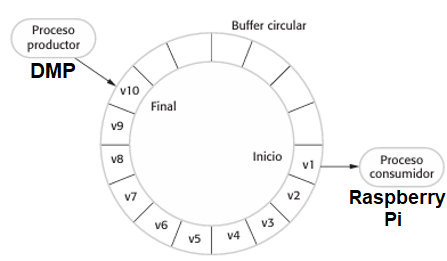
\includegraphics[scale=0.9]{buffer.png}
%	\caption{Representación del buffer interno del MPU como un buffer compartido}
%	\label{fig:buffer}
%\end{figure}

\newpage
La Figura \ref{fig:ejes} muestra los ejes de desplazamiento y la rotación de los sensores MPU. Se colocaron los sensores MPU en la ortesis de modo que el sentido positivo del eje X quedara hacia el frente del operador (quien tiene colocada la ortesis); de acuerdo con esto, el sentido positivo de rotación en el eje Z se obtiene girando el brazo hacia la izquierda del operador; el sentido positivo de rotación en el eje Y se obtiene girando el brazo hacia abajo; y el sentido positivo de rotación en el eje X se obtiene rotando el brazo hacia la derecha.

\begin{figure}[htb]
	\centering
	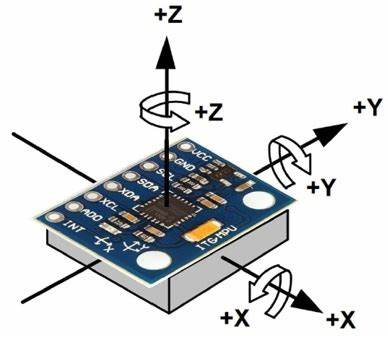
\includegraphics[scale=0.5]{ejes.jpeg}
	\caption{Orientación de los ejes y polaridad de rotación de los sensores MPU}
	\label{fig:ejes}
\end{figure}

Se eligieron los valores de referencia de modo que la salida del sensor en el inicio del proceso de medir la orientación fuera $X=0, Y=0, Z=0$ para el giroscopio y $X=0, Y=0, Z=-9.8$ para el acelerómetro, debido a la constante de la aceleración de la gravedad g = -9.8  $m/s^2$. De acuerdo con lo anterior, al procesar los datos por el DMP, la salida deseada en el inicio del proceso de medir la orientación sería $\theta_x = 0°,\theta_y = 0°,\theta_z = 0°$.

Si el sensor se encuentra en estado de reposo (no existe ninguna fuerza externa que lo mueva), se espera que al leer datos de él, los valores no cambien; en la práctica, estos valores pueden variar debido a interferencias como el ruido externo. De modo que se calcula un valor medio cuyo error (la diferencia entre la medición del sensor en estado de reposo y el valor medio) sea menor que un error máximo aceptable; con base en la experiencia, se eligió un error máximo de 0.1 $\degree/s$ para el giroscopio, y 0.1 $m/s$ para el acelerómetro.

Para obtener dicho valor medio, se utilizó un control proporcional-integral (PI), en el cual se escribe el valor medido por el sensor en los registros de referencia (offset registers), y se compara dicho valor con la siguiente medición del sensor (con el último offset escrito en los registros de referencia aplicado a la nueva medición), para determinar el error; este proceso termina cuando el error obtenido se encuentra dentro del rango previamente establecido.

La Figura \ref{fig:calibracion} muestra el proceso de calibración del sensor. A cada medición se le aplicó el control PI para corregir el error. Para permitir que se establezca un valor apropiado, este proceso se repite 600 veces, un valor elegido basado en la experiencia. Después de que termina el ciclo, se compara el siguiente valor del sensor con los valores de referencia en los registros para determinar el error. Si éste es mayor que el error máximo aceptado, se repite el proceso.

Para que la calibración sea adecuada y se obtenga una medición confiable, el sensor debe de encontrarse en el estado de reposo mencionado anteriormente.

\begin{figure}[htb]
	\centering
	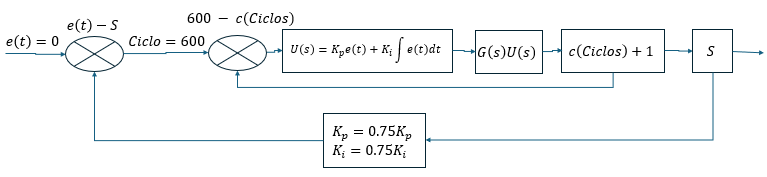
\includegraphics[scale=0.8]{calibracion.png}
	\caption{Diagrama a bloques del proceso de calibración del sensor}
	\label{fig:calibracion}
\end{figure}

\newpage
Posteriormente, se debe de cargar el firmware del procesador \cite{userguideMotionDriver}. Este proceso debe de realizarse cada vez que se encienda el sensor. Aunque no se indique explícitamente, el hecho de que el firmware deba de ser cargado cada vez que se inicie el sensor sugiere que la memoria que contiene el firmware del sensor es una memoria volátil. La memoria está formada por 8 bancos, en los que se carga el firmware proporcionado por InvenSense \cite{userguideMotionDriver}. 

Después de esto, se habilita el DMP y el buffer FIFO escribiendo el valor 1 en el bit FIFO\_EN (Bit 6) del registro 106 indicado en la Figura \ref{fig:fifoen} para la lectura de datos.

\begin{figure}[htb]
	\centering
	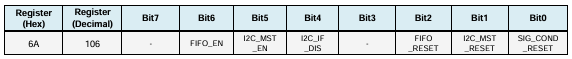
\includegraphics[scale=1]{fifoenable.png}
	\caption{Registro User Control del MPU, donde se encuentra el bit (Bit6) para activar el buffer FIFO}
	\label{fig:fifoen}
\end{figure}

\subsubsection{Medición}

El algoritmo utilizado por el DMP para obtener la orientación, no es de dominio público; en el Capítulo \ref{cap:anexos}, se describe el posible algoritmo utilizado por el DMP. Por otro lado, InvenSense, el desarrollador del sensor, ofrece un conjunto de bibliotecas para trabajar con el DMP \cite{userguideMotionDriver}.

%La Figura muestra el proceso general para obtener la orientación del sensor. Primero, se obtiene en el buffer FIFO la orientación obtenida por el DMP, representada internamente por un cuaternión. El cuaternión es rápidamente computable y evita problemas que se producen al girar más de 90°, como el bloqueo del cardán. Posteriormente, se obtiene el vector de gravedad; este permite calcular la aceleración de la gravedad que experimenta el sensor en los 3 ejes, para tomarlo como sesgo y corregir la medición. Por último, se convierte lo antes calculado a valores de Euler, en radianes, y finalmente, dichos valores son convertidos a su equivalente en grados, que son los que se utilizan para indicar la orientación del sensor.

%\begin{figure}[htb]
%	\centering
%	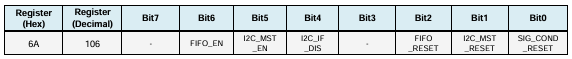
\includegraphics[scale=1]{fifoenable.png}
%	\caption{Determinación de la orientación del sensor}
%	\label{fig:orientacion}
%\end{figure}

El DMP representa internamente la orientación por medio de cuaterniones unitarios. Son rápidamente computables, y evitan problemas que se producen al girar más de 90\degree, como el bloqueo del cardán.

El cuaternión es de la forma:.

\begin{equation}
	q = a + b\hat{i} + c\hat{j} + d\hat{k}
	\label{eq:eqcuaternion}
\end{equation}

Donde $a, b, c, d$ son las componentes del cuaternión que describe la rotación actual del sensor.

Para poder obtener la rotación del sensor, se utilizó la formula que obtiene las nuevas componentes de un vector si se le aplica una rotación descrita por un cuaternión, la cual es la siguiente:

\begin{equation}
	v' = q\cdot v\cdot q*
	\label{eq:rotacioncuaternion}
\end{equation}

Donde $v'$ es el nuevo vector con la rotación aplicada, y $q*$ es el cuaternión conjugado, de la forma:

\begin{equation}
	q* = a - b\hat{i} - c\hat{j} - d\hat{k}
	\label{eq:eqcuaternionconj}
\end{equation}

De acuerdo con los valores de referencia definidos para el acelerómetro ($X=0, Y=0, Z=-9.8$), el vector de gravedad es $g = (0, 0, -1)$.

Se sustituyó en la ecuación \ref{eq:rotacioncuaternion} $v$ por el vector de gravedad. Al resolver para $v'$, se obtuvieron las siguientes ecuaciones para obtener cada componente:

\begin{equation}
	v'_x = 2\cdot(x \cdot z - w \cdot y)
	\label{eq:componentex}
\end{equation}

\begin{equation}
	v'_y = 2\cdot(w \cdot x + y \cdot z)
	\label{eq:componentey}
\end{equation}

\begin{equation}
	v'_z = w^2 - x^2 - y^2 + z^2
	\label{eq:componentez}
\end{equation}

Para obtener los ángulos entre el vector $v'$ y los ejes $x$, $y$, $z$ definidos cuando se calibró el sensor (es decir, aquella orientación del sensor en la que la salida del DMP es $\theta_x = 0°,\theta_y = 0°,\theta_z = 0°$), se utilizaron las siguientes ecuaciones:

\begin{equation}
	\theta_x = \tan^{-1}\frac{v'_y}{v'_z}
	\label{eq:angulox}
\end{equation}

\begin{equation}
	\theta_y = \tan^{-1}\frac{v'_x}{\sqrt{v'^2_y + v'^2_z}}
	\label{eq:anguloy}
\end{equation}

\begin{equation}
	\theta_z = \tan^{-1}\frac{q_x \cdot q_y + q_w \cdot q_z}{1 - 2 \cdot (q_x^2 + q_y^2)}
	\label{eq:anguloz}
\end{equation}

Si el sensor se encuentra boca abajo (es decir, la componente Z del vector de gravedad apunta en el sentido positivo del eje Z), es necesario invertir el sentido de la inclinación en el eje Y. Si el valor de la inclinación en el eje Y es positivo, el valor se corrige a $\pi - v'_y$; si es negativo, el valor se ajusta a $-\pi - v'_y$.

Los ángulos obtenidos $\theta_x$, $\theta_y$, $\theta_z$, son la orientación del sensor.

\subsection{Localización}

Para obtener la posición (x, y, z) en el espacio, se utilizan las

\subsection{Visualización}

La empresa requirió que se mostrara en una interfaz gráfica un brazo en 2D controlado con los ángulos calculados de la cinemática inversa.

Para desarrollar la aplicación, se utilizó el framework Qt, en cual se implementaron las etapas de Sensado y Localización en C++. La interfaz se implementó en QML, un lenguaje declarativo que facilitó el desarrollo de la interfaz.

El proceso de lectura de datos del sensor se ejecuta constantemente, lo que puede bloquear los procesos de la interfaz y que ésta deje de responder para el usuario. Para evitar dicho problema, se colocó dicho proceso de lectura de datos en un hilo; éste permite que un subproceso pueda ejecutarse de forma concurrente con otros subprocesos. Para que el hilo de captura de datos pueda comunicar las lecturas a la interfaz, y que éstas puedan ser visualizadas en la interfaz gráfica, se utiliza el paso de mensajes; Qt permite enviar mensajes entre hilos a través de señales. De este modo, también se evitan problemas de concurrencia si ambos hilos intentan acceder a la misma variable donde se almacenan los datos de los sensores.

En la Figura \ref{fig:interfaz} se observa el brazo en 2D; puede notarse que se indica el plano que está siendo visualizado; esto puede ser configurado con el botón arriba a la izquierda. También puede observarse la posición del efector final determinada por la etapa de localización. La gráfica está graduada, de modo que se puede apreciar la precisión del modelo.

\begin{figure}[htb]
	\centering
	
\includegraphics[scale=0.5]{interfaz.jpg}
	\caption{Interfaz gráfica de usuario mostrada en la pantalla táctil de la Raspberry Pi}
	\label{fig:interfaz}
\end{figure}

\subsection{Referencia}

La empresa requirió que se utilizara un brazo robótico en 3D diseñado por la propia empresa, e incluido en el software SettDev, para ser empleado como referencia del movimiento realizado por la ortesis. La Figura \ref{fig:referencia} muestra el brazo en 3D diseñado por la propia empresa. Puede notarse que en la parte superior hay controles deslizantes. La empresa requirió que estos controles mostraran los ángulos utilizados como referencia, es decir, que los ángulos aplicados para controlar el movimiento del brazo en 3D, se mostraran numéricamente en los controles deslizantes.

\begin{figure}[htb]
	\centering
	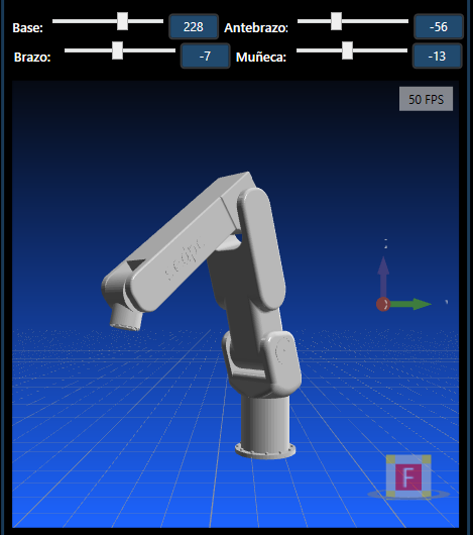
\includegraphics[scale=0.8]{referencia.png}
	\caption{Brazo en 3D utilizado como referencia en el software SettDev}
	\label{fig:referencia}
\end{figure}

\subsection{Almacenamiento}

Finalmente, los ángulos calculados por la red se almacenaron en un archivo. El formato para almacenar los archivos es el que muestra la Figura \ref{fig:formatoarchivo}.

\begin{figure}[htb]
	\centering
	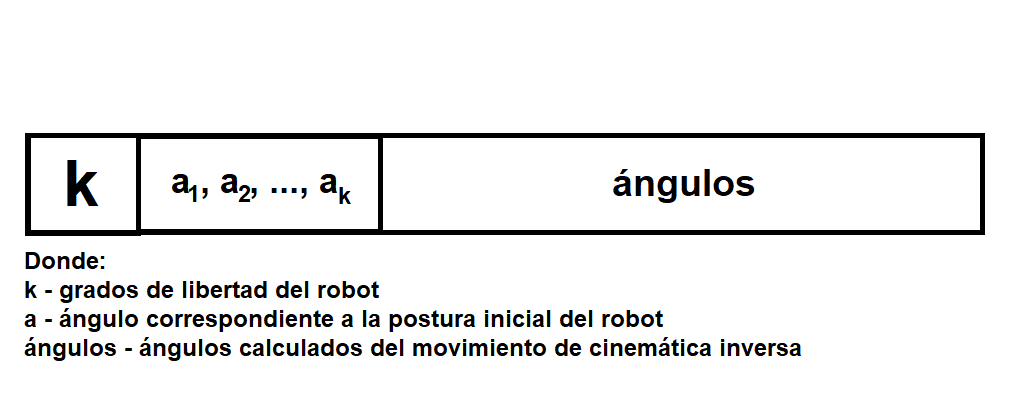
\includegraphics[scale=0.6]{formatoarchivo.png}
	\caption{Formato del archivo que guarda los datos de movimiento}
	\label{fig:formatoarchivo}
\end{figure}

El contenido del archivo se describe como sigue:

\begin{enumerate}
	\item El primer byte guarda la cantidad $k$ de ángulos de cinemática inversa calculados para el robot con $k$ grados de libertad
	\item Los siguientes $k$ bytes almacenan los ángulos de inclinación de la postura inicial del robot. Esta no necesariamente debe de corresponder con la postura inicial del brazo del operador, ya que lo que se controla en el brazo robótico, es el desplazamiento desde la posición inicial.
	\item El resto del contenido del archivo son los ángulos calculados para el problema de la cinemática inversa.
\end{enumerate}

De acuerdo con el mapa de registros \cite{registermap}, el tipo de dato del valor del ángulo de inclinación medido es de 2 bytes con signo. Esto quiere decir que el archivo aumenta en 18 bytes de información por cada instante en el que se mida la inclinación del dispositivo.

\newpage
\section{Fase de ejecución}

\subsection{Lectura}

Se implementó la funcionalidad en el software SettDev para leer y reproducir un archivo. La Figura \ref{fig:cargaarchivo} muestra el módulo de carga de un archivo. El programa permite abrir un cuadro de diálogo para seleccionar un archivo del equipo, de tipo .bin. Cuando se da clic al botón ``Abrir'' y se cierra el archivo, el programa verifica la extensión del archivo. Posteriormente, comienza a leer los datos del archivo.

\begin{figure}[htb]
	\centering
	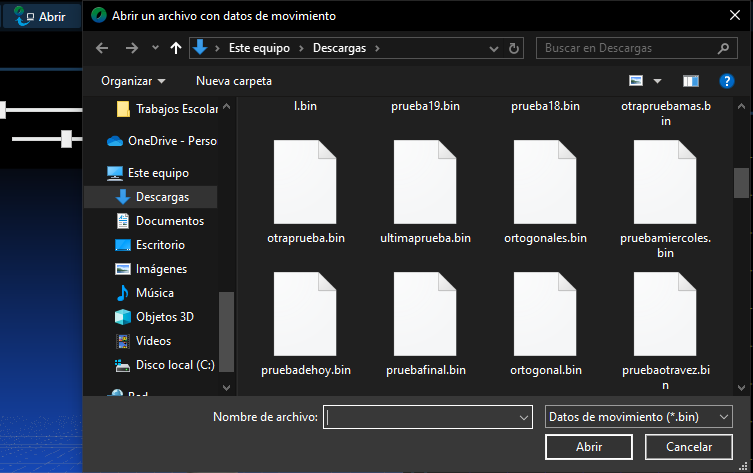
\includegraphics[scale=0.65]{cargaarchivo.png}
	\caption{Módulo de carga de archivo implementado en SettDev}
	\label{fig:cargaarchivo}
\end{figure}

\subsection{Transmisión}

Se desarrolló e implementó la comunicación entre el software SettDev y el PLC para transmitir los datos leídos desde el archivo. El PLC-Kaab de SEDPC se controla y comunica utilizando datagramas; éstos se envían por medio del protocolo UDP, y tienen un formato de trama específico, que es el que se muestra en la Figura \ref{fig:tramaPLC} obtenida del documento . La trama comienza con un encabezado (Header) que siempre contiene el valor 8A, seguido de algunas indicaciones para el PLC, como el proceso Fuente del que provienen los datos, el proceso de Destino, e indicaciones internas (Internal Indications). Luego, se indica un comando (Command), un subcomando (Subcommand), la indicación de algún Error producido, y la longitud $n$ de los datos por enviar (Largo). Los siguientes $n$ bytes contienen la información a enviar (Data). Por último, se calcula un Checksum como medio de comprobación de errores; si se produce algún error, el PLC no reproduce el datagrama enviado. Se utilizan identificadores con valores numéricos para indicar la Fuente o Destino (el proceso) que envía o recibe los datos, así como el comando y subcomando por ejecutar.

\begin{figure}[htb]
	\centering
	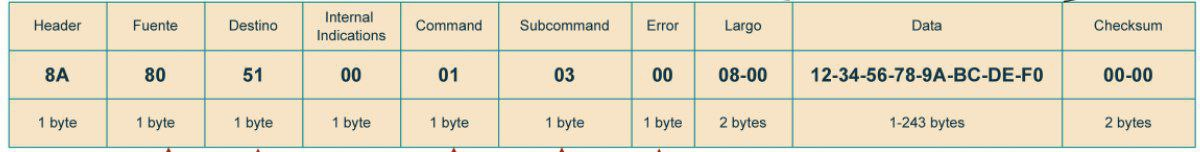
\includegraphics[scale=0.4]{tramaPLC.jpg}
	\caption{Formato de trama utilizado por el PLC-Kaab}
	\label{fig:tramaPLC}
\end{figure}

Para elaborar la trama, se tomó como referencia la que genera un módulo desarrollado por SEDPC en SettDev para controlar servomotores. En dicha interfaz, existen controles deslizantes que indican los ángulos enviados al PLC; los valores son transmitidos al dar clic a un botón ``Enviar''. El contenido de la trama generado por este módulo es el que se muestra en la Figura . Los campos Fuente y Destino contienen el valor 06, que hace referencia al proceso de Interfaz Gráfica de Usuario (el software SettDev, y el software contenido en el PLC); el comando 02 indica una escritura de datos en el PLC (en este caso, el nuevo ángulo); y el subcomando 06 indica una entrada de datos digitales (los datos contenidos en la trama). Como los errores se comprueban antes de enviar la trama, el campo Error siempre contiene el valor 00; el campo Largo indica que el tamaño del campo Data es de 19 bytes. En dicho campo, los datos se indican como sigue:

\begin{enumerate}
	\item Byte 1: Tipo de motor (el valor 1 identifica a los servomotores)
	\item Bytes 3-7: Nuevo ángulo en formato Little Endian
	\item Bytes 8-11: Pulso mínimo en formato Little Endian
	\item Bytes 12-15: Pulso máximo en formato Little Endian
	\item Bytes 16-19: Ángulo máximo en formato Little Endian
\end{enumerate}

En el formato Big Endian, que es el que comúnmente se utiliza para representar un valor digital, los bytes de izquierda a derecha se ordenan desde el más significativo hasta el menos significativo. En el formato Little Endian, este orden se invierte.

\subsection{Reproducción}

Los datos se interpretaron por el PLC y se reprodujeron en los servomotores conectados al mismo. Se añadió una tarjeta de control de motores desarrollada por SEDPC que utiliza transistores MOSFET para modular el ángulo recibido por el PLC en una señal de ancho de pulso. El PLC-Kaab utilizado cuenta con 8 ranuras para conectar en cada una de ellas la línea de señal de control de cada motor a controlar. En la Figura se muestran las ranuras, en las que se han conectado 4 líneas de señal de control de 4 servomotores. Las últimas dos ranuras son las líneas de alimentación de voltaje que alimentan a todos los servomotores conectados en paralelo.

\newpage
\chapter{Resultados}

\newpage
\renewcommand{\bibname}{Referencias}
\bibliographystyle{IEEEtran}
\bibliography{referencias}

\newpage
\chapter{Anexos}\label{cap:anexos}

% Fin del documento
\end{document}